%%%%%%%%%%%%%%%%%%%%%%%%%%%%%%%%%%%%%%%%%%%%%%%%%%%%%%%%%%%%%%%%%%%%%%%%%%%%%%%%
%2345678901234567890123456789012345678901234567890123456789012345678901234567890
%        1         2         3         4         5         6         7         8

% Key links for ICRA2020
% CFP: https://www.icra2020.org/call-for-papers
% PaperPlaza: https://ras.papercept.net/conferences/scripts/start.pl
% Author Guidelines: http://ras.papercept.net/conferences/support/tex.php

\documentclass[letterpaper, 10 pt, conference]{ieeeconf}
%\documentclass[a4paper, 10pt, conference]{ieeeconf}

% This command is only needed if you want to use the \thanks command
\IEEEoverridecommandlockouts

\overrideIEEEmargins

%In case you encounter the following error:
%Error 1010 The PDF file may be corrupt (unable to open PDF file) OR
%Error 1000 An error occurred while parsing a contents stream. Unable to analyze the PDF file.
%This is a known problem with pdfLaTeX conversion filter. The file cannot be opened with acrobat reader
%Please use one of the alternatives below to circumvent this error by uncommenting one or the other
%\pdfobjcompresslevel=0
%\pdfminorversion=4

% See the \addtolength command later in the file to balance the column lengths
% on the last page of the document

% The following packages can be found on http:\\www.ctan.org
%\usepackage{graphics} % for pdf, bitmapped graphics files
%\usepackage{epsfig} % for postscript graphics files
%\usepackage{mathptmx} % assumes new font selection scheme installed
%\usepackage{times} % assumes new font selection scheme installed
%\usepackage{amsmath} % assumes amsmath package installed
%\usepackage{amssymb}  % assumes amsmath package installed

\usepackage{graphicx}
\graphicspath{{figures/}}
\usepackage{caption}
\usepackage{tabularx}
\usepackage{booktabs}

\usepackage{lipsum}

\title{
    \LARGE \bf%
    A Reduced-Order Approach to Assist with Reinforcement Learning for Underactuated Robotics
}

\author{
    J\'er\'emy Augot$^{1,2}$, Aaron J Snoswell$^{2}$ and Surya P. N. Singh$^{2}$
% <-this % stops a space
\thanks{
    $^{1}$ Ecole CentraleSup\'elec, Paris, France
}%
\thanks{
    $^{2}$The Robotics Design Lab at The University of Queensland, Brisbane, Australia
}%
}

\begin{document}

\maketitle
\thispagestyle{empty}
\pagestyle{empty}

%%%%%%%%%%%%%%%%%%%%%%%%%%%%%%%%%%%%%%%%%%%%%%%%%%%%%%%%%%%%%%%%%%%%%%%%%%%%%%%%
\begin{abstract}

\lipsum[1]

\end{abstract}

%%%%%%%%%%%%%%%%%%%%%%%%%%%%%%%%%%%%%%%%%%%%%%%%%%%%%%%%%%%%%%%%%%%%%%%%%%%%%%%%
\section{INTRODUCTION}

\lipsum[1-2]

\begin{figure}[ht]
    
    \centering
    
    \begin{minipage}[b]{0.49\linewidth}
        \centering
        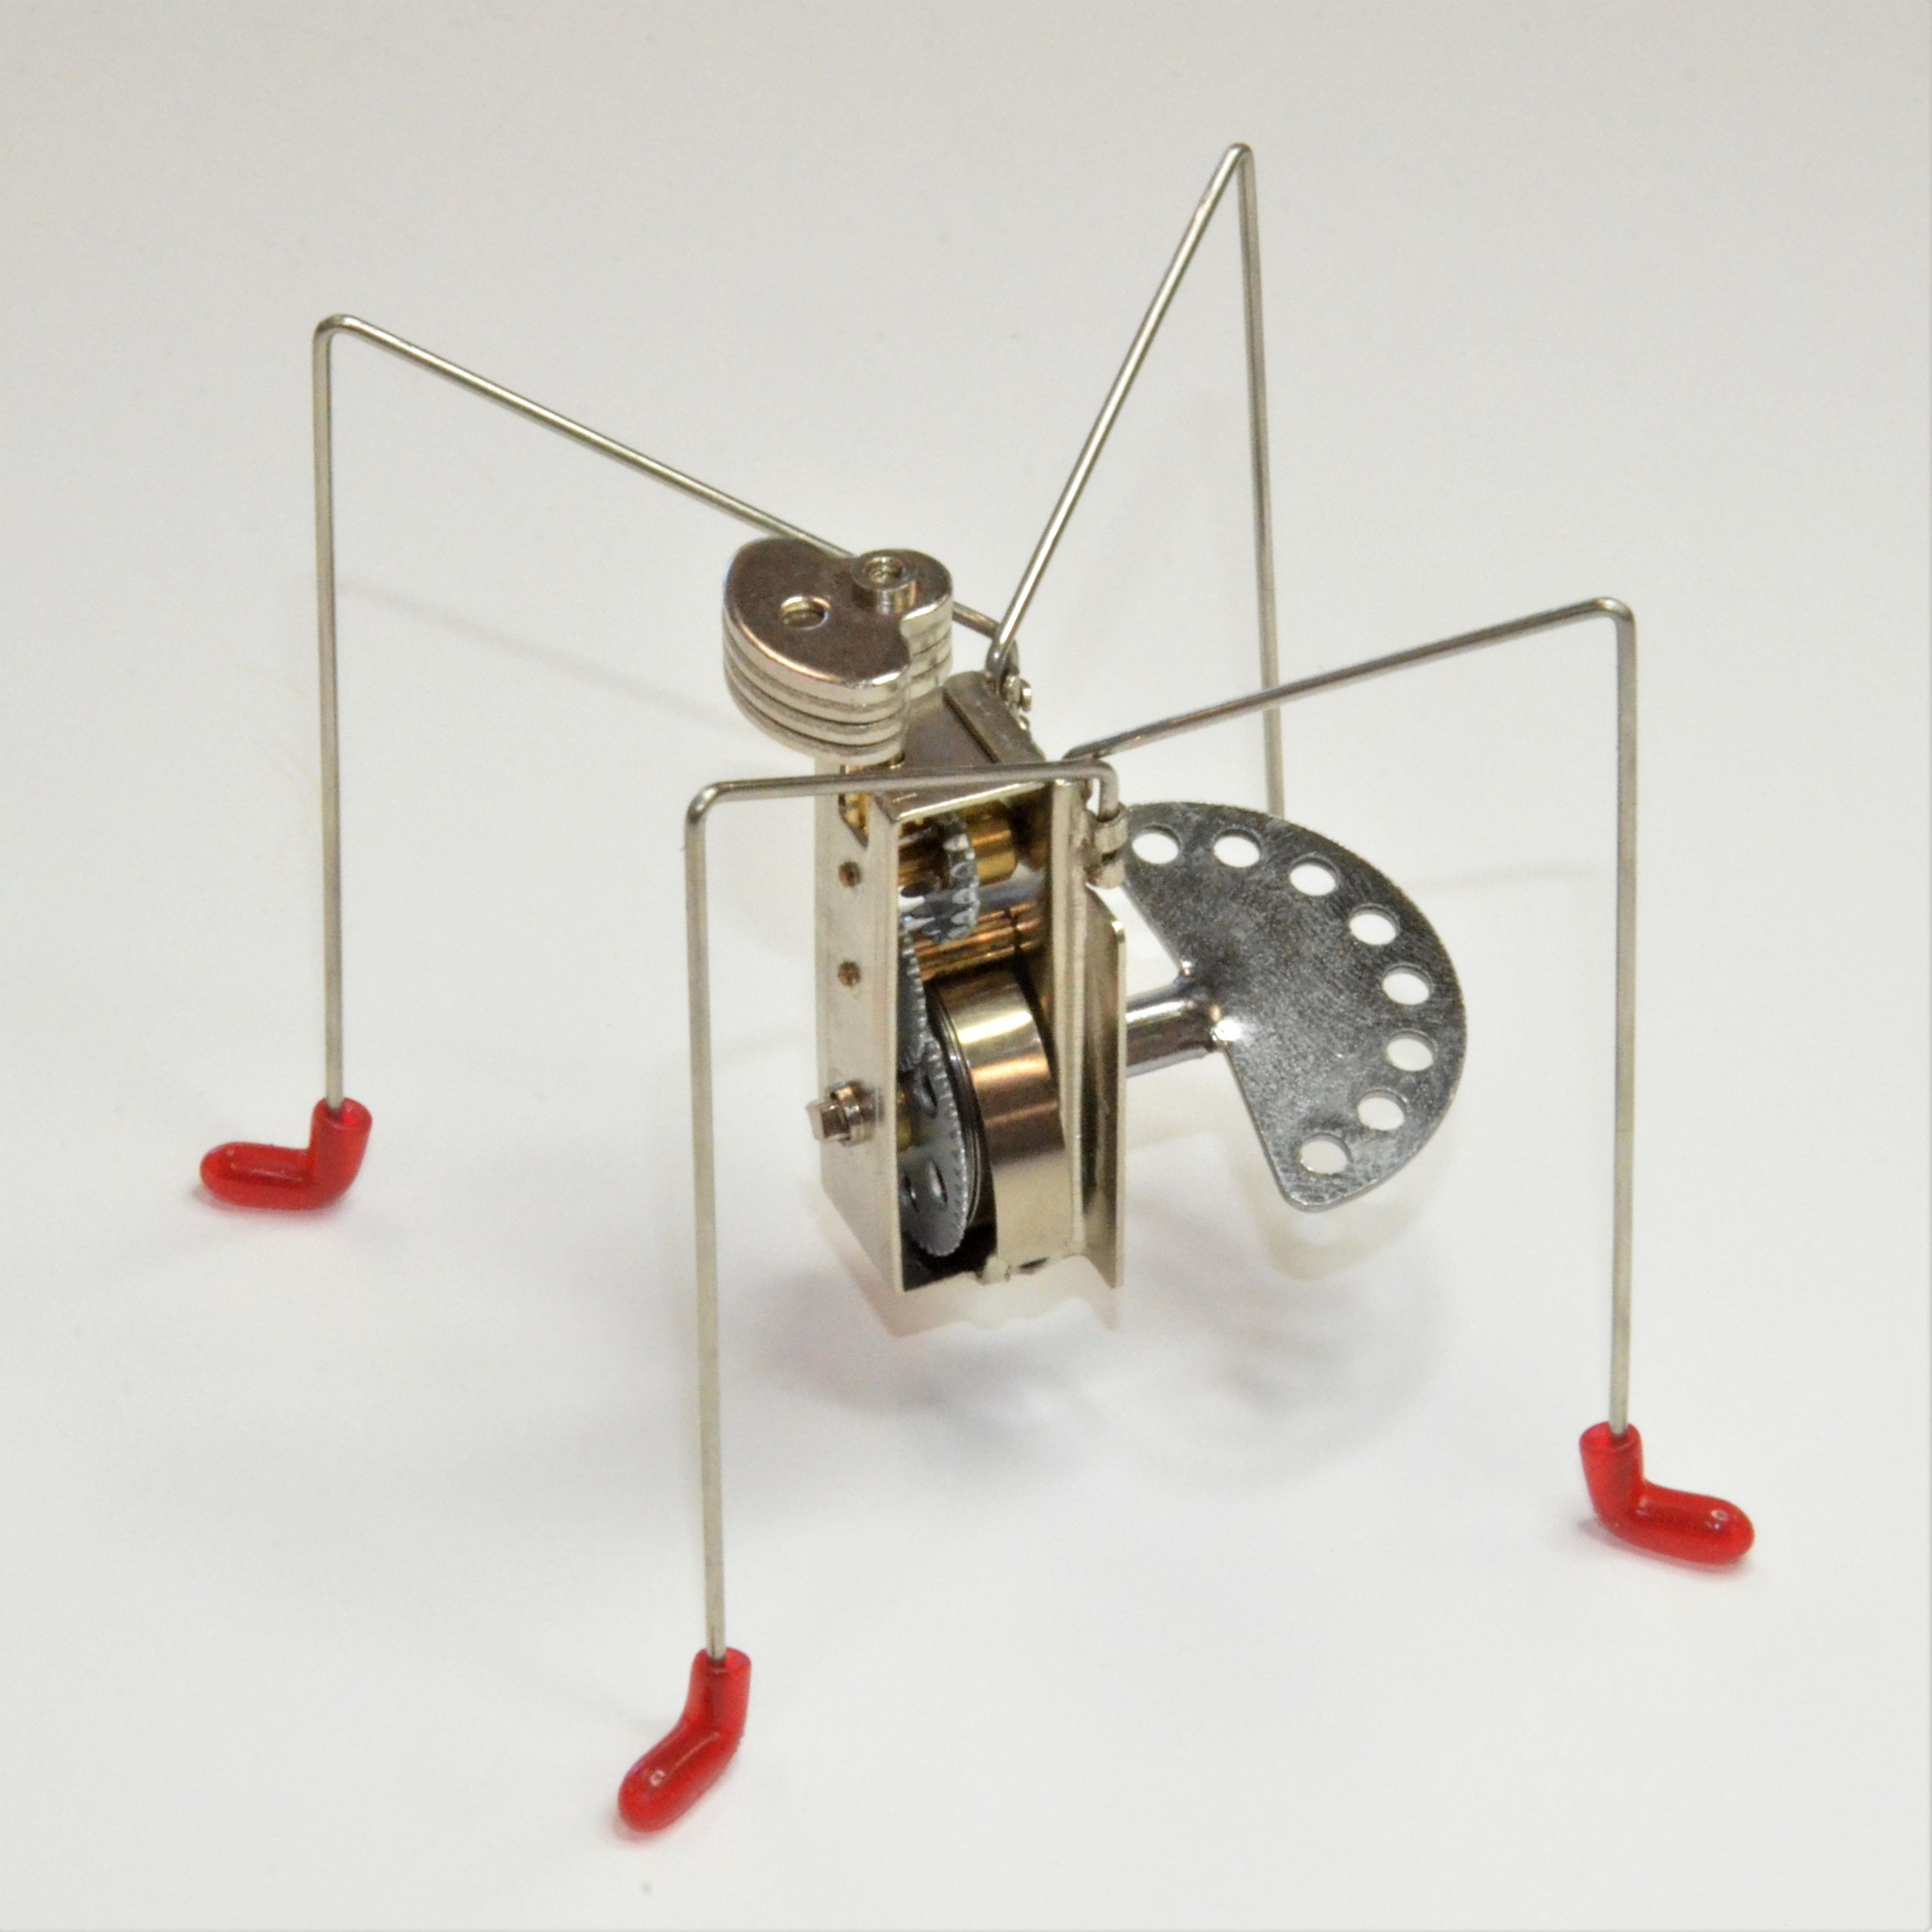
\includegraphics[width=\linewidth]{katita}
    \end{minipage}
    \begin{minipage}[b]{0.49\linewidth}
        \centering
        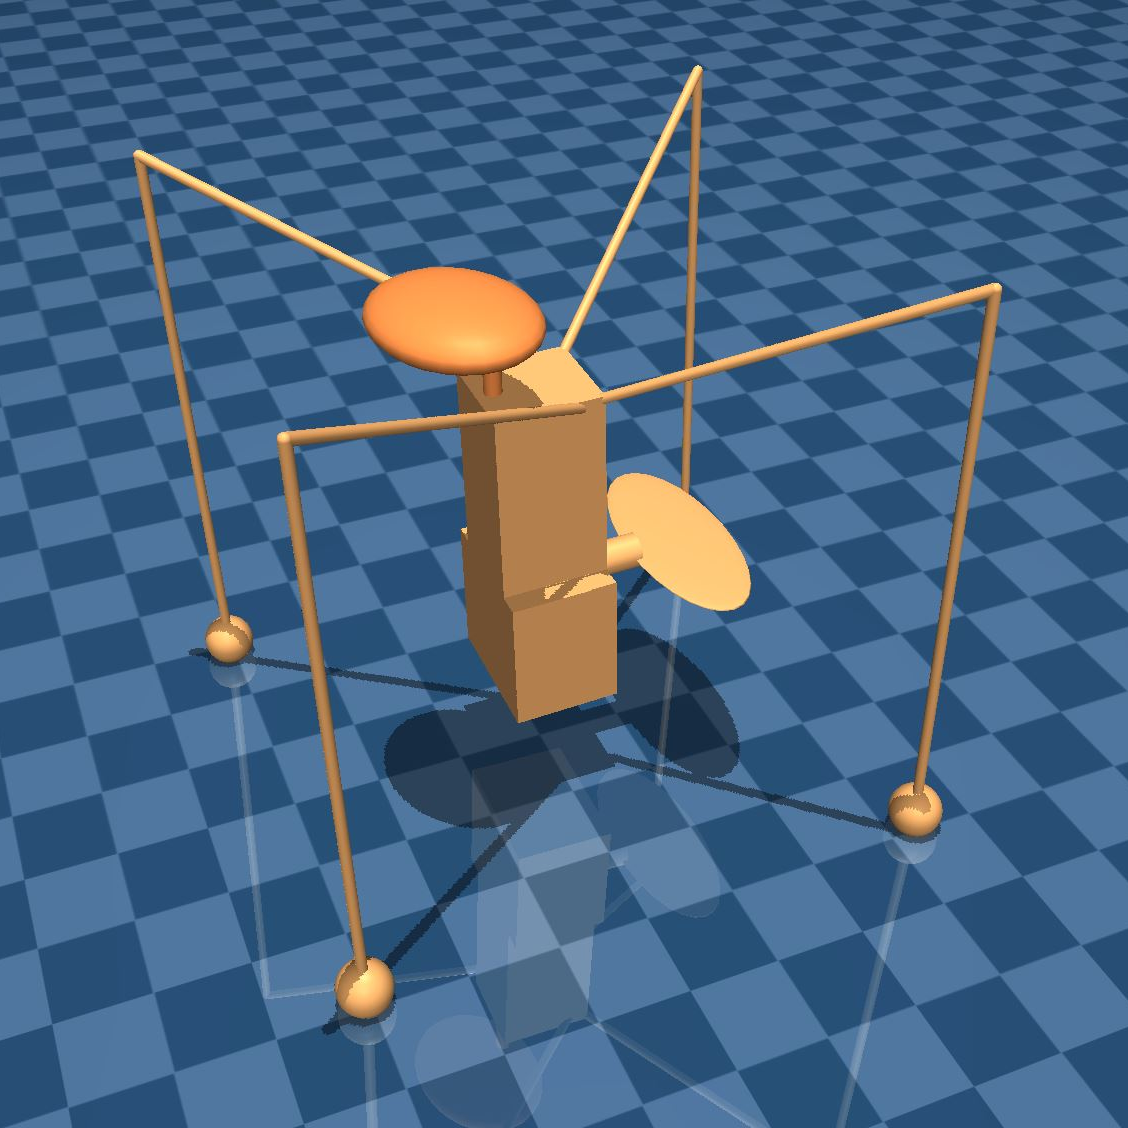
\includegraphics[width=\linewidth]{jitterbug}
    \end{minipage}
    
    \caption{
        The wind-up children's toy `Katita' (left) was the inspiration for our underactuated `Jitterbug' continuous control task (right).
        In the simulated robot the wind-up spring is replaced with a controlled single degree-of-freedom motor.
        The simulated robot retains the (non functional) wind-up crank to more closely mimic the mass distribution of the real toy.
    }
    \label{fig:leader}
    
\end{figure}

\lipsum[1-4]

\section{RELATED WORK}

\subsection{Reinforcement Learning}

\subsection{Deep Deterministic Policy Gradients (DDPG)}

\subsection{Advantage Actor-Critic (A2C)}

\subsection{Proximal Policy Optimization (PPO)}

\subsection{DeepMind Control Suite}

\subsection{Under-actuated Control}

\lipsum[1-2]

\begin{figure}[ht]
    \centering
    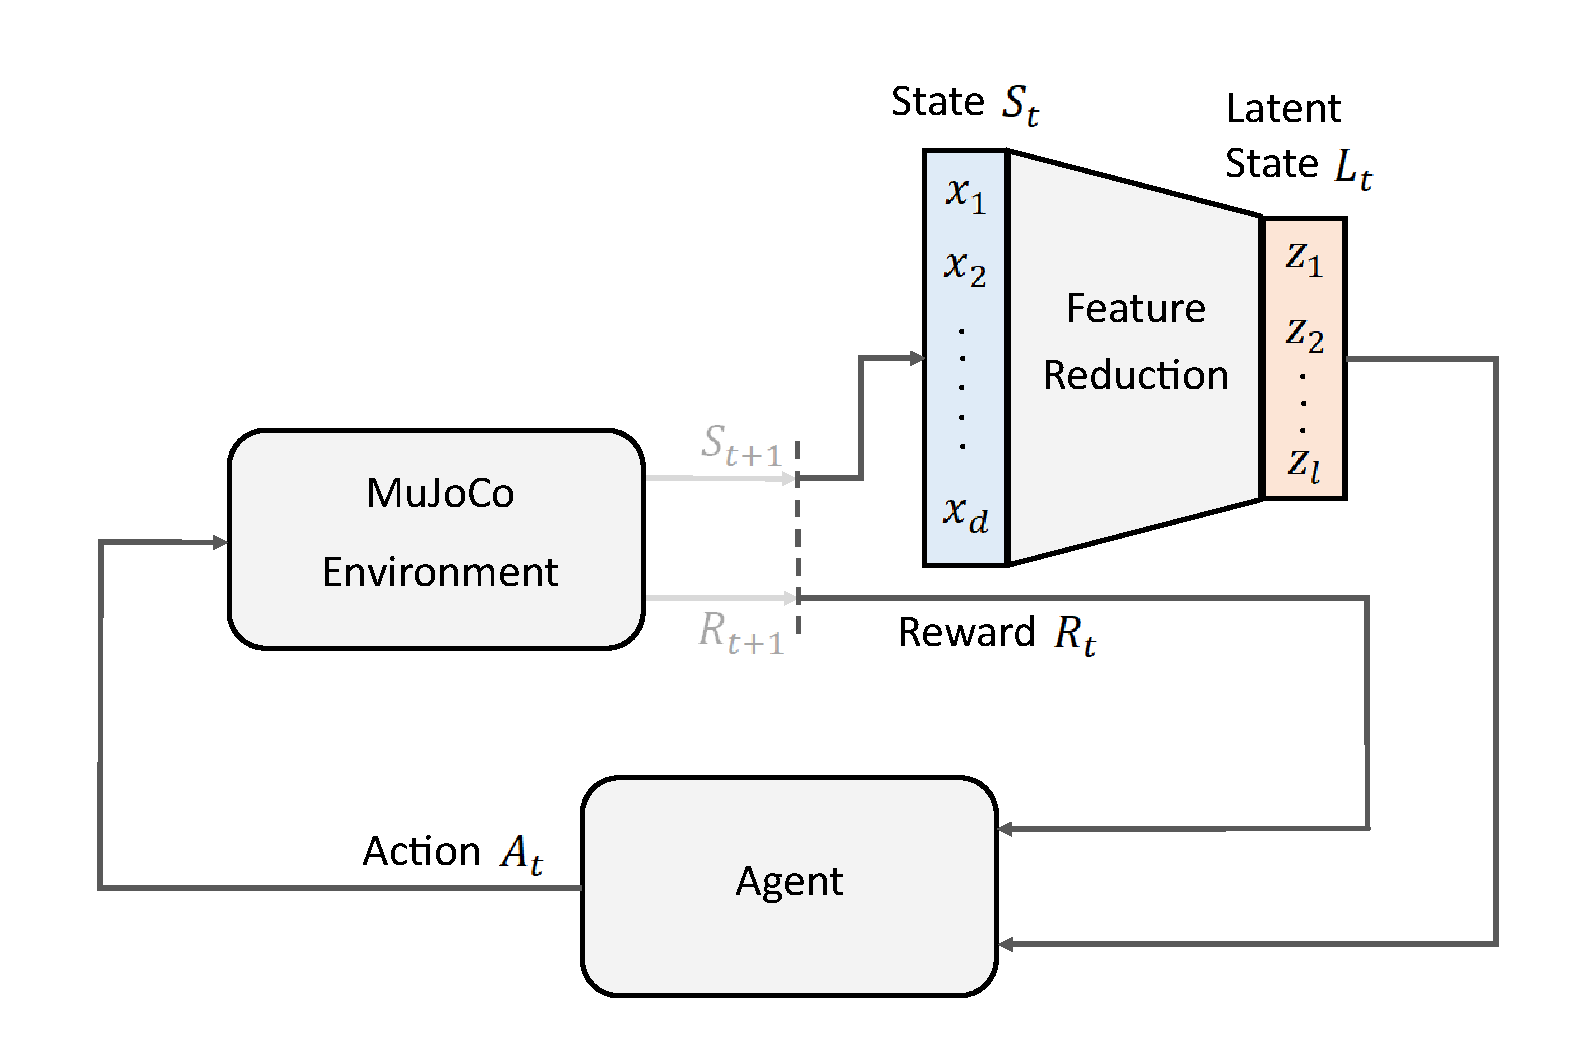
\includegraphics[width=\linewidth]{fig-system-arch}
    \caption{
        The architecture of our system.
    }
    \label{fig:system-arch}
\end{figure}

\section{METHOD}

\lipsum[1-9]

\section{THE JITTERBUG ENVIRONMENT}

\lipsum[1-9]

\section{EXPERIMENTS}

\begin{figure}[ht]
    \centering
    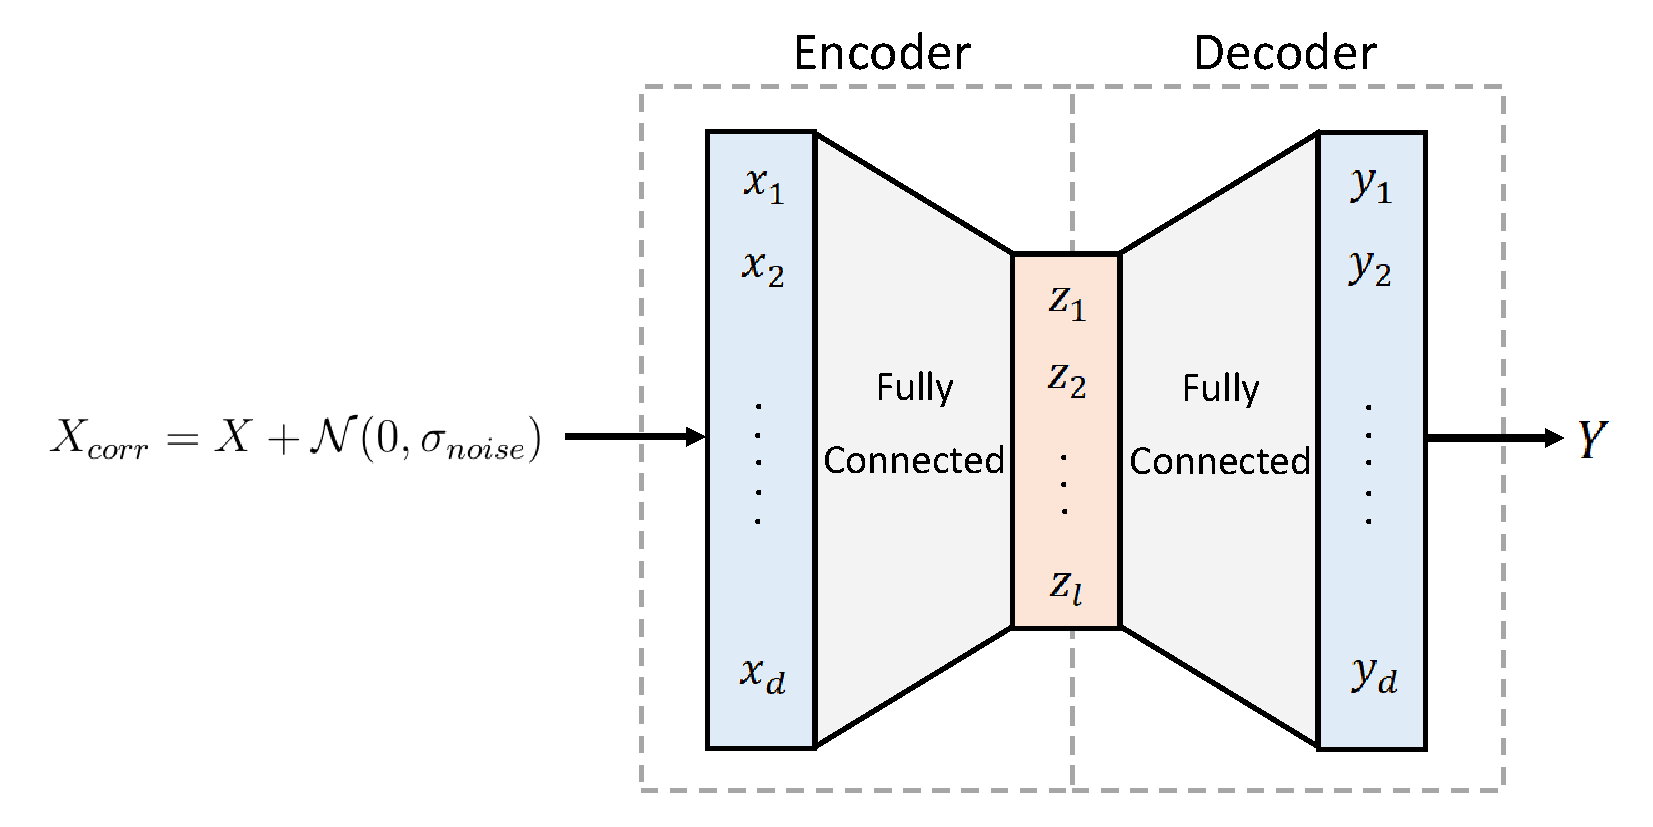
\includegraphics[width=\linewidth]{fig-autoencoder}
    \caption{
        WE used a De-Noising AutoEncoder as a means to learn a reduced-order state representation.
    }
    \label{fig:autoencoder}
\end{figure}

\lipsum[1]

\begin{table*}[t!]
    
    \centering
    \caption{Algorithm Hyper-parameters}
    \label{tab:results}
    \medskip
    
    {\def\arraystretch{1.2}
        \begin{tabularx}{\textwidth}{X rr c rr c rr}
            
            \toprule
            
            & \multicolumn{2}{c}{\% Distance Match} & \phantom{a} & \multicolumn{2}{c}{Feature Vector L2} & \phantom{a} & \multicolumn{2}{c}{Log Likelihood} \\
            
            \cmidrule{2-3} \cmidrule{5-6} \cmidrule{8-9}
            
            & {avg.} & {med.} & & {avg.} & {med.} & & {avg.} & {med.} \\
            
            \midrule
            
            MaxEnt (Ours) &
            56.74 & 57.52 &  & 5.145E3 & 1.270E3 &  & 4.360E-121 & 2.932e-121 \\
            
            MaxEnt \cite{Ziebart2008} &
            38.03 & 31.36 &  & 172.406E3 & 178.043E3 &  & $-\infty$ & $-\infty$ \\
            
            MaxEnt (Length-binned ensemble) &
            60.12 & 62.13 &  & 3.388E3 & 1.662E3 &  & 1.050e-14 & 8.733e-15 \\
            
            MaxEnt ($k$-means ensemble) &
            65.58 & 73.68 &  & 1.132E3 & 562.29 &  & 3.74E-119 & 2.8228e-119 \\[10pt]
            
            
            Shortest Path &
            52.10 & 50.54 &  & 2.679E3 & 995.400 &  & {-} & {-} \\
            
            Logistic Regression &
            52.45 & 50.18 &  & {-} & {-} &  & {-} & {-} \\
            
            \bottomrule
            
        \end{tabularx}
    }
    
\end{table*}

\lipsum[1-9]

\begin{figure}[h]
    \centering
    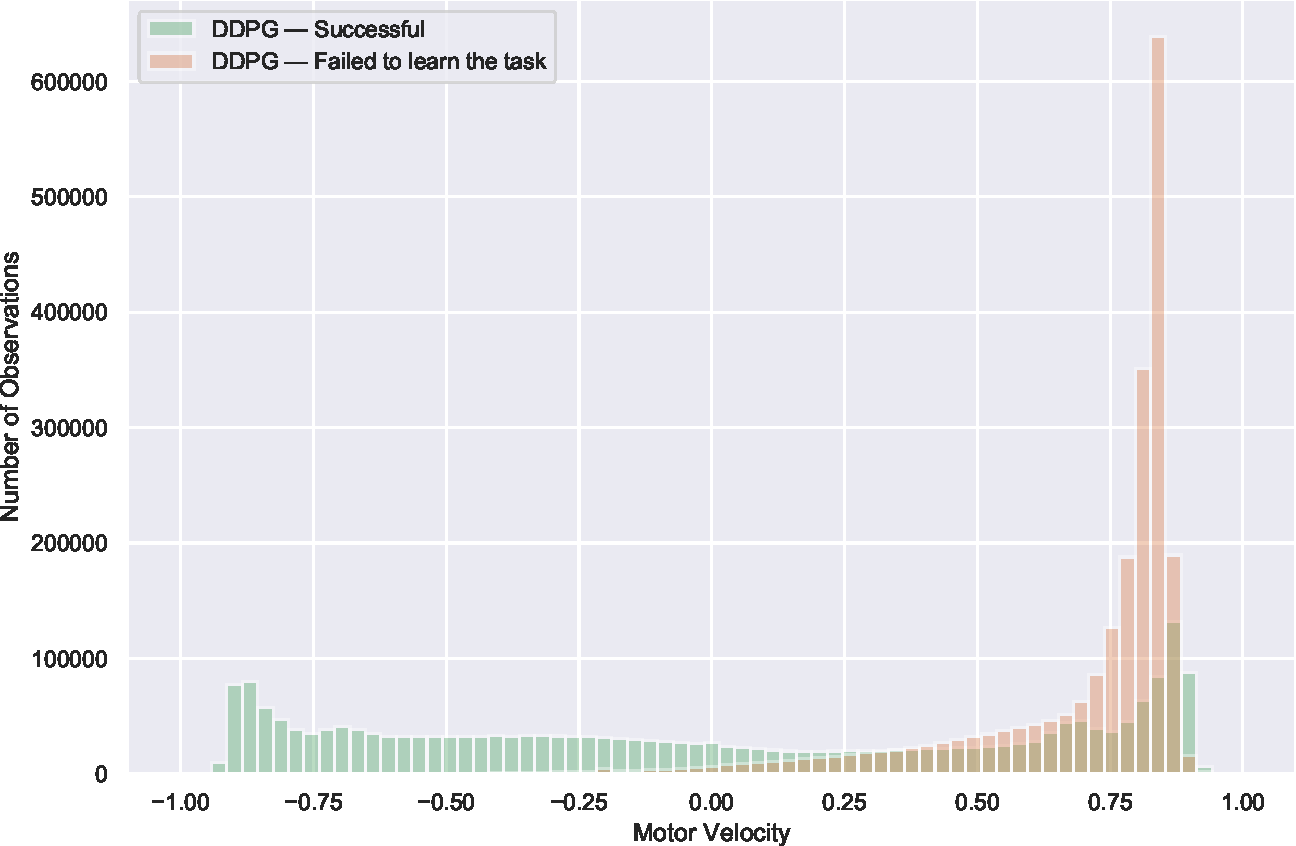
\includegraphics[width=\linewidth]{fig-motor-hist}
    \caption{
        Characterising successful policy behaviours.
        A histogram of motor velocities.
    }
    \label{fig:motor-hist}
\end{figure}

\begin{figure*}[p]
    
    \centering
    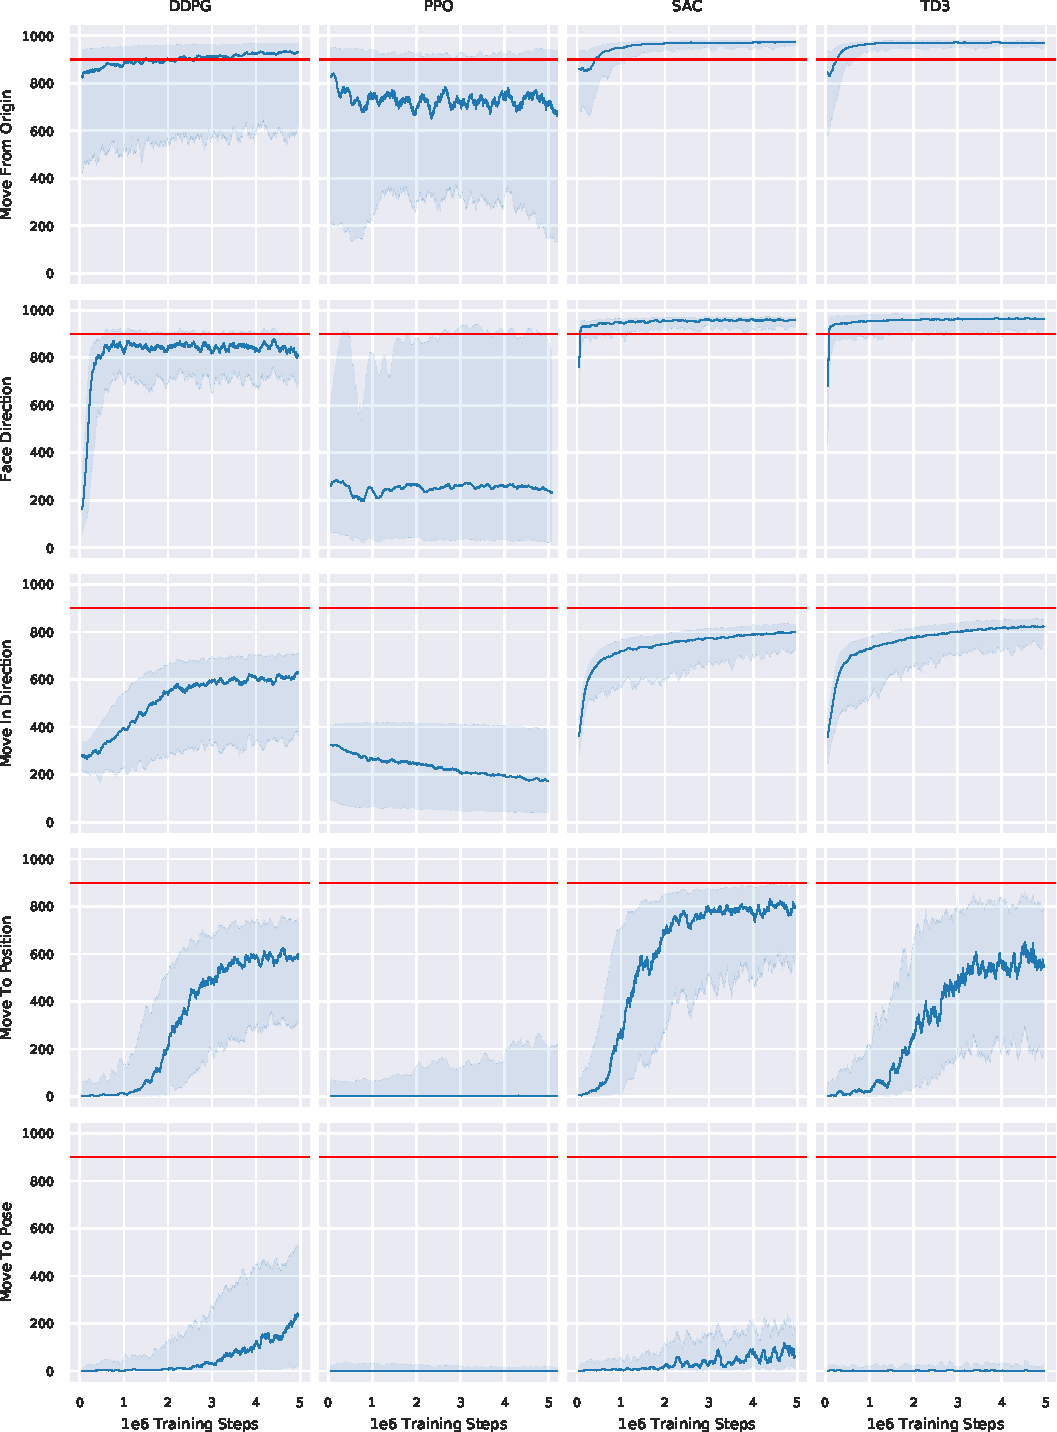
\includegraphics[width=\textwidth]{fig-rl-perf}
    
    \captionsetup{margin=10pt}
    \caption{
        Comparison of RL algorithms over environment training steps.
        We show median (solid line) and the first and third quartiles (shaded area) across 10 random seeds in each figure.
        All plots are filtered with a $10e^3$ step moving average filter.
    }
    
    \label{fig:rl-perf}
\end{figure*}

\section{DISCUSSION}

\lipsum[1]

\section{CONCLUSION}

\lipsum[1]

%\addtolength{\textheight}{-12cm}   % This command serves to balance the column lengths
                                  % on the last page of the document manually. It shortens
                                  % the textheight of the last page by a suitable amount.
                                  % This command does not take effect until the next page
                                  % so it should come on the page before the last. Make
                                  % sure that you do not shorten the textheight too much.

%%%%%%%%%%%%%%%%%%%%%%%%%%%%%%%%%%%%%%%%%%%%%%%%%%%%%%%%%%%%%%%%%%%%%%%%%%%%%%%%



%%%%%%%%%%%%%%%%%%%%%%%%%%%%%%%%%%%%%%%%%%%%%%%%%%%%%%%%%%%%%%%%%%%%%%%%%%%%%%%%



%%%%%%%%%%%%%%%%%%%%%%%%%%%%%%%%%%%%%%%%%%%%%%%%%%%%%%%%%%%%%%%%%%%%%%%%%%%%%%%%
\section*{APPENDIX}

\lipsum[1]

\section*{ACKNOWLEDGMENT}

\lipsum[1]

%%%%%%%%%%%%%%%%%%%%%%%%%%%%%%%%%%%%%%%%%%%%%%%%%%%%%%%%%%%%%%%%%%%%%%%%%%%%%%%%

\begin{thebibliography}{99}

\bibitem{c1} G. O. Young, Synthetic structure of industrial plastics (Book style with paper title and editor), in Plastics, 2nd ed. vol. 3, J. Peters, Ed.  New York: McGraw-Hill, 1964, pp. 1564.

\end{thebibliography}


\end{document}
